\documentclass[e2_tp1_main.tex]{subfiles}

\begin{document}


\section{Rendimiento}

Un par\'ametro fundamental de una fuente de tensi\'on regulada es el rango de tensiones de entrada en el cual la salida se encuentra en regulaci\'on. Idealmente, con cualquier tensi\'on igual o supuerior a la de salida se podr\'ia obtener $V_{O\, REG}$, pero la necesidad de llevar a los transistores del circuito a un punto de trabajo apropiado hace que haya una diferencia de tensi\'on m\'inima entre la entrada y la salida. 

Tomando como criterio que el circuito est\'a regulando correctamente si la tensi\'on de salida es un 99\% o m\'as de la que se tiene sin carga, se obtuvieron los datos de la tabla \ref{table:rendimiento}.

\begin{table}[htb!]
\centering
\begin{tabular}{|c||c|c|}
\hline
$V_{O\,REG}$ (V) & $V_I - V_O$ simulada (V) & $V_I - V_O$ medida (V) \\ \hline\hline
9                & 1.263                    & 1.37                   \\ \hline
10               & 1.273                    & 1.37                   \\ \hline
11               & 1.281                    & 1.5                    \\ \hline
12               & 1.286                    & 1.18                   \\ \hline
13               & 1.290                    & 1.29                   \\ \hline
14               & 1.293                    & 1.26                   \\ \hline
15               & 1.295                    & 1.13                   \\ \hline
\end{tabular}
\caption{Rendimiento medido y simulado para distintas tensiones de regulaci\'on}
\label{table:rendimiento}
\end{table}

En promedio, pues, se obtuvo que:

\begin{equation}
	\left\{
	\begin{aligned}
	\Delta V_{MIN\,SIM} &= 1.28V \\ 
	\Delta V_{MIN\,MED} &= 1.3V \\ 
	\end{aligned}
	\right.
\end{equation}



\section{Impedancia de salida}

Una caracter\'istica de una fuente de tensi\'on regulada ideal es que posee impedancia de salida cero, lo cual resultar\'ia en regulaci\'on de carga ideal, es decir: la tensi\'on de salida es la misma para cualquier valor de $R_L$. Desde ya, en la pr\'actica esto es imposible de obtener, pero la realimentaci\'on negativa de este tipo de fuentes permite obtener un valor de $R_O$ lo suficientemente peque\~no como para que sea despreciable en la mayor\'ia de los casos. 

Anal\'iticamente, el valor de $R_O$ se obtiene a partir de la impedancia de salida del circuito amplificador b\'asico $R_{OA}$ y la ganancia de lazo $|T|$:

\begin{equation}
	R_O = \frac{R_{OA}}{1+|T|}
	\label{eq:rout}
\end{equation}

En la ecuaci\'on ~\ref{eq:rout} resulta muy claro por qu\'e la realimentaci\'on negativa mejora esta caracter\'istica del circuito: en lugar de ver directamente la impedancia de salida del circuito amplificador b\'asico, la carga ve a esta impedancia reducida $1+|T|$ veces.\\
El an\'alisis se realizo eligiendo el generados, el amplificador, la re-alimentación de la siguiente manera:
\begin{figure}[H]
  \centering
   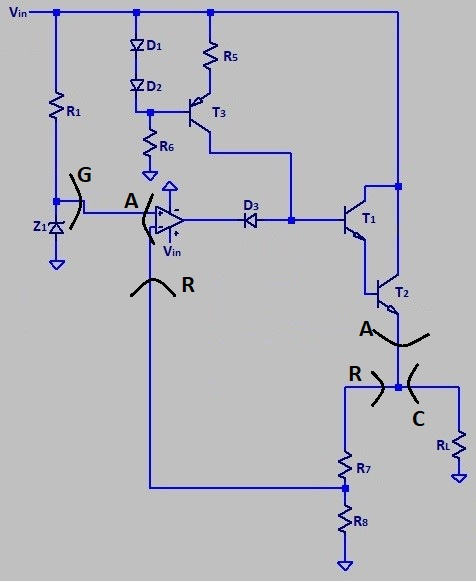
\includegraphics[width=0.45\textwidth]{Analisis.jpg}
   \caption{Elección de etapas}
   \label{fig:CircuitoEtapas}
\end{figure} 
A partir de la figura ~\ref{fig:CircuitoEtapas} podemos observar que la vamos a tener suma de tensión y muestreo de tensión dando una ganancia de re-alimentación $f=\frac{V_1}{V_2}|_{I_1=0}=\frac{R_8}{R_8+R_7}$.
A continuación calculamos la ganancia a lazo abierto con el siguiente circuito:
\begin{figure}[H]
  \centering
   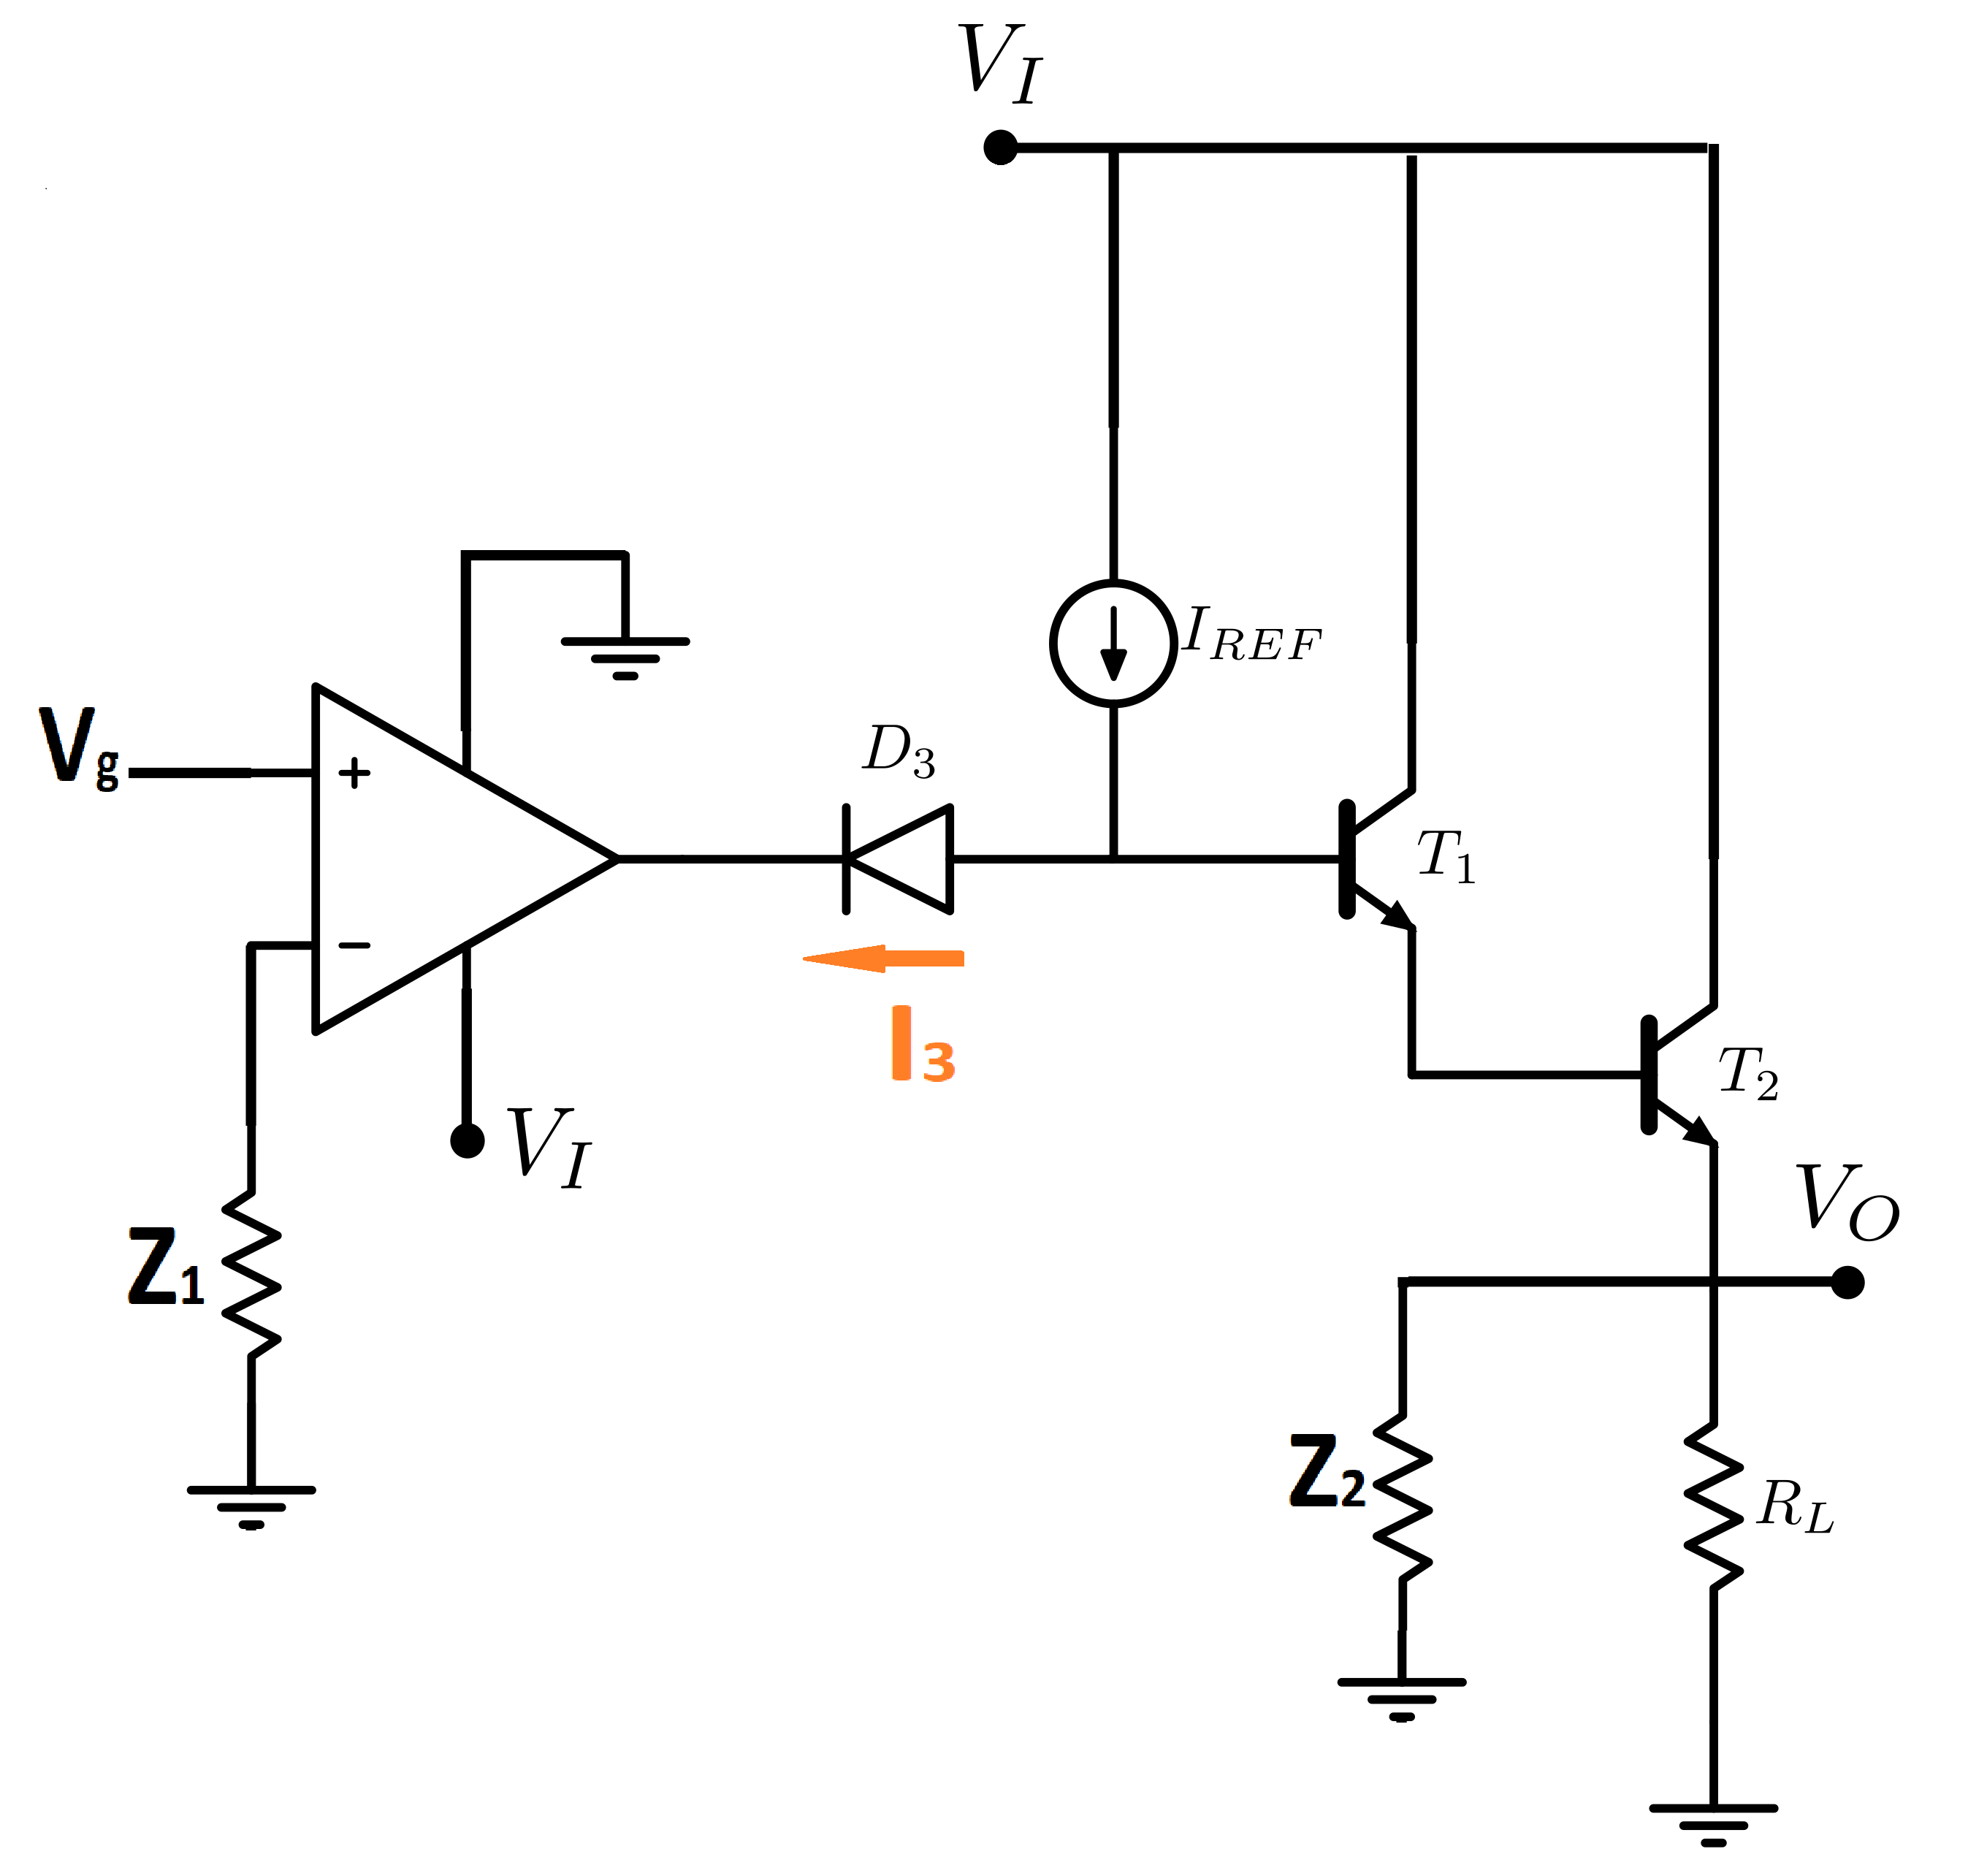
\includegraphics[width=0.45\textwidth]{AmplificadorBasico.png}
   \caption{Elección de etapas}
   \label{fig:AmplificadorBasico}
\end{figure} 
En donde reemplazamos el transistor $T_3$ junto sus correspondientes componentes por una fuente de corriente para simplificar el análisis y remplazamos el generador por un $V_g$ de forma tal que nos queda lo observado por la figura ~\ref{fig:AmplificadorBasico}. De la misma podemos observar que la ganancia a lazo abierto nos va a dar como resultado: 
$$a=\frac{V_2}{V_1}=\frac{(\epsilon{}A_{vol}-V_{D3}-V{BE1}-V{BE2}+I_3R_{out})(Z_2//R_L)(\beta_1+1)(\beta_2+1)}{V_g[R_{out}+(\beta_1+1)(\beta_2+1)(Z_2//R_L)]}$$
Al cual aproximando $(\epsilon{}A_{vol}-V_{D3}-V{BE1}-V{BE2}+I_3R_{out})(Z_2//R_L)(\beta_1+1)(\beta_2+1)\simeq\epsilon{}A_{vol}$, dado que todas las demás variables son chicas en comparación a $\epsilon{}A_{vol}$ la cual se encuentra multiplicada por la ganancia del amplificador del operacional y $\epsilon$ que tiene mayor valor que el resto. Ademas aproximamos $V_g[R_{out}+(\beta_1+1)(\beta_2+1)(Z_2//R_L)]\simeq(\beta_1+1)(\beta_2+1)(Z_2//R_L)$ dado que $R_{out}$ va a ser despreciable en comparación a $(\beta_1+1)(\beta_2+1)(Z_2//R_L)$ quedando:
$$a=\frac{\epsilon{}A_{vol}(Z_2//R_L)(\beta_1+1)(\beta_2+1)}{V_g(\beta_1+1)(\beta_2+1)(Z_2//R_L)}=\frac{\epsilon{}A_{vol}}{V_g}$$
Dado que $\epsilon{}=V_g\frac{R_{ent}}{R_{ent}+Z_1}$ tenemos que el valor final va a ser $a=\frac{A_{vol}R_{ent}}{R_{ent}+Z_1}$.
Finalmente, dado que $Z_1=R_8//R_7$ y $Z_2=R_8+R_7$ obtenemos que $a\simeq{}A_{vol}$ porque $\frac{R_{ent}}{R_{ent}+Z_1}\simeq1$.

Para obtener la impedancia de salida calculamos la impedancia de salida dada por los transistores $T_1$ y $T_2$ los cuales están en una configuración DARLINGTON, utilizando el modelo incremental obtenemos $R_{out}=\frac{\frac{r_{\pi1}}{1+\beta_1}+r_{\pi2}}{1+\beta_2}$ y dado que $r_{\pi}=(1+\beta)\frac{V_T}{I_{cq}}$ estas van a variar acorde a la corriente de polarización y la temperatura a la cual se este usando el transistor. 

Finalmente obtuvimos anal\'iticamente que:

\begin{equation}
	\left\{
	\begin{aligned}
	|T| &\simeq{}A_{vol}\frac{R_8}{R_7+R_8}\simeq{}99,18\,dB\\
	R_{OA} &\simeq{}R_L//Z_2//Z_{outCascode}
	\end{aligned}
	\right.
\end{equation}

Remiti\'endonos nuevamente a la ecuaci\'on \ref{eq:rout}, resulta entonces en el caso típico donde $I_{cq2}=1,5\,A$ y estando a temperatura ambiente, que:
$$R_O \simeq 379\times 10^{-6}\Omega$$
En el peor caso donde $R_{OA}\simeq{}Z_2$ tenemos que:
$$R_O \simeq 557\times 10^{-3}\Omega$$

Para simular y medir este valor, se estudi\'o la regulaci\'on de carga del circuito. Si la impedancia de salida fuese cero, deber\'ia cumplirse que tanto para corriente 0 como para cualquier valor de $I_O$, la tensi\'on de salida es la misma. A medida que $R_O$ aumenta, m\'as cae la tensi\'on a medida que aumenta la corriente. Se decidi\'o pues calcular $R_O$ a partir de:

\begin{equation}
	R_O = \frac{V_O|_{I_O=0} - V_O|_{I_O=I_{O\,1}}}{I_{O\,1}}
\end{equation} 

Si bien, en principio, esta ecuaci\'on es v\'alida para cualquier par de valores de $\Delta V_O$ y $\Delta I_O$, se decidi\'o utilizar $I_{O\,1}$=1A, debido a que los valores de $\Delta V_O$ en regulaci\'on son muy peque\~nos, y por lo tanto dif\'iciles de medir con precisi\'on con el instrumental que se ten\'ia disponible, lo cual incurre en un gran error porcentual en la determinaci\'on del mismo, que se propaga proporcionalmente a $R_O$. A pesar de que esta forma se ignora el hecho de que la impedancia de salida cambia con la carga, dado que cambia la polarizaci\'on de todos los diodos y transistores del circuito, se consider\'o que se incurrir\'ia as\'i en menos error que tratando de medir las variaciones de unos pocos mV (o inferiores) que ocurren en valores similares de corriente.

\begin{table}[!htb]
\centering
\begin{tabular}{|c|c|c|}
\hline
$V_{O\,REG}$ (V) & $R_O$ simulada ($\Omega$) & $R_O$ medida ($\Omega$) \\ \hline\hline
9                & $3 \times 10^{-6}$        & $6 \times 10^{-2}$      \\ \hline
15               & $2 \times 10^{-6}$        & $2 \times 10^{-2}$      \\ \hline
\end{tabular}
\caption{Valores simulados y medidos para la impedancia de salida}
\label{table:rout}
\end{table}



\end{document}